% Created 2020-12-04 Fri 12:37
% Intended LaTeX compiler: pdflatex
\documentclass[presentation]{beamer}
\usepackage[utf8]{inputenc}
\usepackage[T1]{fontenc}
\usepackage{graphicx}
\usepackage{grffile}
\usepackage{longtable}
\usepackage{wrapfig}
\usepackage{rotating}
\usepackage[normalem]{ulem}
\usepackage{amsmath}
\usepackage{textcomp}
\usepackage{amssymb}
\usepackage{capt-of}
\usepackage{hyperref}
\usetheme{UoB}
\author{Mark Blyth}
\date{\textit{[2020-12-07 Mon]}}
\title{Continuation and polynomials}
\hypersetup{
 pdfauthor={Mark Blyth},
 pdftitle={Continuation and polynomials},
 pdfkeywords={},
 pdfsubject={},
 pdfcreator={Emacs 27.1 (Org mode 9.3)}, 
 pdflang={English}}
\begin{document}

\maketitle

\section{Background}
\label{sec:org352cf30}
\begin{frame}[label={sec:orga372be9}]{Week's goal}
Code up a numerical continuation algo
\vfill
\begin{itemize}
\item Goal: use BSplines for the continuation
\end{itemize}
\vfill
\begin{itemize}
\item Result: skimmed a pile of papers
\begin{itemize}
\item Dropped down a rabbit hole, but a more relevant one than usual!
\end{itemize}
\end{itemize}
\end{frame}

\section{Collocation}
\label{sec:orga5b9df8}
\begin{frame}[label={sec:org0c1eef3}]{Continuation coding}
Following the continuation algo described in Kuznetsov Elements
\vfill
\begin{itemize}
\item Uses Lagrange polynomials as continuation basis functions
\item It states we should choose zeros of Legendre polynomials as collocation mesh
\begin{itemize}
\item Provides maximal accuracy at collocation points
\end{itemize}
\end{itemize}
\end{frame}

\begin{frame}[label={sec:org18a46bb}]{Lagrange polynomials}
Not provided by SciPy in the required form, so I need to implement them myself
\vfill
\begin{itemize}
\item \(f(t) = \sum \beta_j l_j(t)\)
\item \(l_j(t) = \prod_{m\neq j} \frac{t - t_m}{t_j-t_m}\)
\item Inefficient: \(\mathcal{O}(n^2)\) flops for each \(t\) evaluation
\end{itemize}
\vfill
Barycentric Lagrange polynomials:
\begin{itemize}
\item Denominator is \(t\)-independent, so pre-compute it as weights \(w_i\)
\item Compute \(t\)-dependent product \(\omega(t)\) at each evaluation
\item \(f(t) = \omega(t)\sum \beta_iw_i \frac{1}{t - t_j}\)
\item \(w_i = \frac{1}{\prod_{k\neq i} (t_i - t_k)}\)
\item \(\omega(t) = \prod(t - t_k)\)
\item \(\mathcal{O}(n)\) flops for each \(t\) evaluation
\end{itemize}
\end{frame}

\begin{frame}[label={sec:org61a0ce3},plain]{Lagrange polynomials and CBC collocation}
Lagrange polynomials are heavily susceptible to Runge's phenomenon

\begin{center}
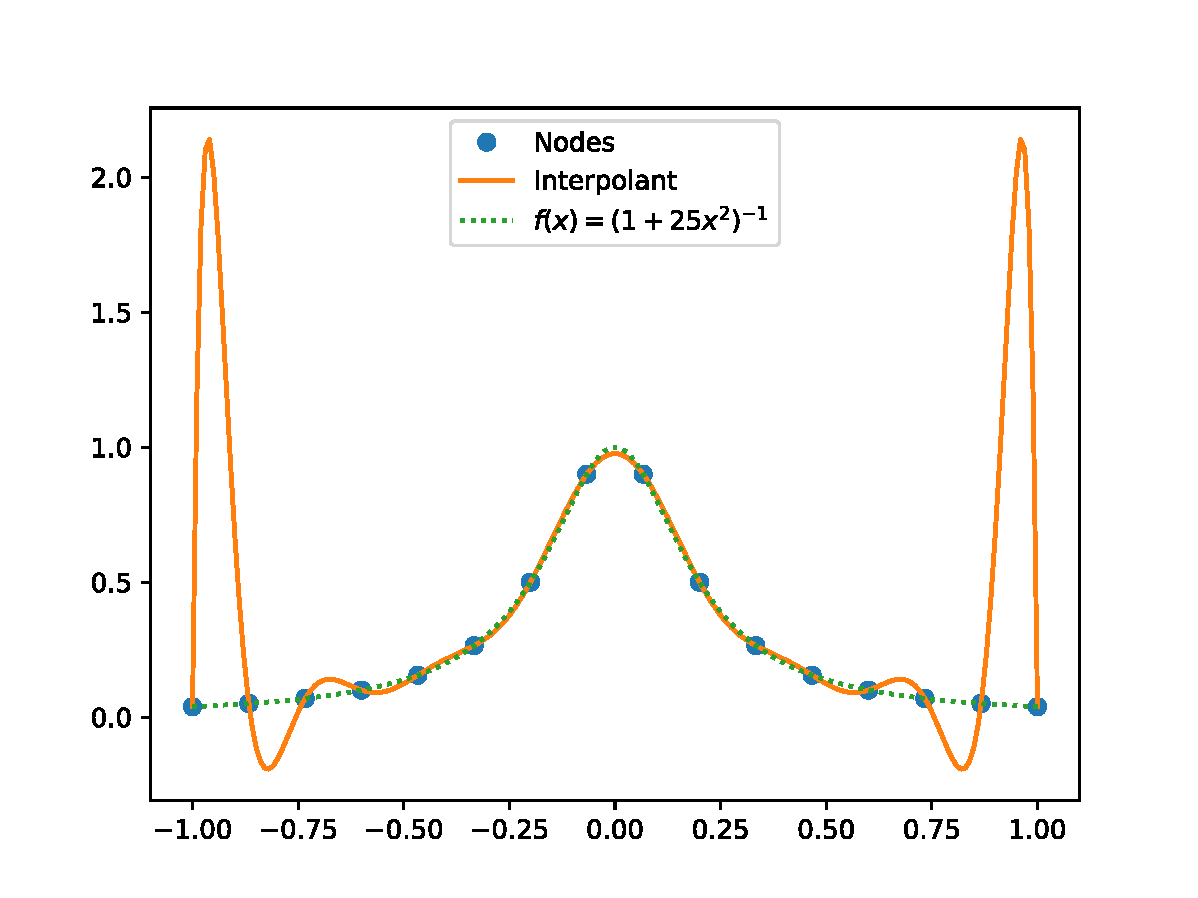
\includegraphics[width=\linewidth]{./runge.pdf}
\end{center}
\end{frame}

\begin{frame}[label={sec:org427d7ea}]{Runge's phenomenon and Lagrange polynomials}
\begin{itemize}
\item Standard setup:
\begin{itemize}
\item Use Lagrange interpolating polynomials
\item Use zeros of Legendre polynomials as collocation mesh
\end{itemize}
\end{itemize}
\vfill
\begin{itemize}
\item Claimed to give best accuracy \emph{at} collocation points, but what about between them?
\begin{itemize}
\item If we're using the result as a control target, Runge's phenomenon is not acceptable
\item We need accuracy \emph{between} collocation points, just as much as \emph{at} meshpoints
\end{itemize}
\end{itemize}
\end{frame}

\begin{frame}[label={sec:org3fd4402}]{Runge's phenomenon}
Idea: use Chebyshev nodes as collocation points
\begin{itemize}
\item Minimises \(\|f(t)-p(t)\|_\infty\), the largest deviation between a continuous function \(f\) and its polynomial approximation \(p\)
\item Minimises Runge's phenomenon!
\item Could use Chebyshev nodes for Lagrange collocation in CBC
\item Equivalently, could use Chebyshev polynomials as collocation basis functions
\begin{itemize}
\item Chebyshev polynomial collocation exists!
\item The paper on Chebyshev collocation looks very useful; yet to read it
\end{itemize}
\item Will \emph{hopefully} make the collocated solution a good control target
\end{itemize}
\end{frame}

\begin{frame}[label={sec:org0d8ef61}]{Two notes}
\begin{itemize}
\item Splines let us control the order of the polynomials by splitting the function up into separate polynomial segments; splines therefore also control Runge's phenomenon
\end{itemize}
\vfill
\begin{itemize}
\item Lagrange, Chebyshev polynomials form an orthonormal basis
\begin{itemize}
\item Could use them in place of Fourier or BSplines for Galerkin CBC
\item Based on Runge's phenomenon, they might not be a good choice for neuronal signals
\item Could work very for `simpler' (Duffing) systems
\end{itemize}
\end{itemize}
\end{frame}

\begin{frame}[label={sec:org2487660}]{Main take-aways so far}
\begin{itemize}
\item Currently coding up standard numerical continution with Lagrange polynomial collocation, as per Kuznetsov Elements
\end{itemize}
\vfill
\begin{itemize}
\item For CBC applications, we don't want Runge's phenomenon
\begin{itemize}
\item Chebyshev might be better than Lagrange polynomials for CBC
\item Splines might be better than interpolating polynomials
\end{itemize}
\end{itemize}
\vfill
\begin{itemize}
\item Could use Lagrange, Chebyshev polynomials for either `standard' Galerkin CBC discretisation, or CBC collocation
\end{itemize}
\end{frame}

\section{RKHS}
\label{sec:org492c638}
\begin{frame}[label={sec:org52ee4dd},plain]{NODYCON reviewer 2}
Their suggestion: fit a `proper' model of the system, and use that as a surrogate
\begin{itemize}
\item Issue: requires us to come up with some generic model that we can fit to the system; hard to do if we don't yet know what the system does
\item Refinement: combine system identification and surrogate modelling
\begin{itemize}
\item Simultaneously produce and refine a model of the system, and use that as a surrogate for further continuation steps
\end{itemize}
\end{itemize}
\vfill
\begin{itemize}
\item Brought to mind reproducing kernel Hilbert spaces
\begin{itemize}
\item Kernel method, like GPR: projects into a feature space; models are linear in feature space, nonlinear in original space
\item Used in ML for fitting regression models; would work as a surrogate
\item Used in NLD for system modelling and identification
\item If it's both a regression model and a system identification method, maybe it's exactly what we need?
\end{itemize}
\end{itemize}
\vfill
I don't yet understand anything about RKHS. Going to work through some papers and figure out if they'll be useful or relevant.
\end{frame}

\section{Next steps}
\label{sec:org62808c4}

\begin{frame}[label={sec:orgbf5204e}]{Next steps}
\begin{itemize}
\item Keep coding up `standard' numerical continuation
\end{itemize}
\vfill
\begin{itemize}
\item Try Legendre, Chebyshev, BSpline, \dots{} CBC collocation with both standard continuation and CBC
\begin{itemize}
\item Compare solution curves for collocation, Galerkin, and various basis functions
\end{itemize}
\end{itemize}
\vfill
\begin{itemize}
\item Try Galerkin CBC again
\end{itemize}
\vfill
\begin{itemize}
\item See if RKHS do anything interesting
\end{itemize}
\end{frame}

\begin{frame}[label={sec:org893ffb5},plain]{References}
\begin{itemize}
\item Bouvrie, Jake, and Boumediene Hamzi. "Kernel methods for the approximation of nonlinear systems." SIAM Journal on Control and Optimization 55.4 (2017): 2460-2492.
\item Nejib, Hamza, Okba Taouali, and Nasreddine Bouguila. "Identification of nonlinear systems with kernel methods." 2016 IEEE International Conference on Systems, Man, and Cybernetics (SMC). IEEE, 2016.
\item Hamzi, Boumediene, and Houman Owhadi. "Learning dynamical systems from data: a simple cross-validation perspective." arXiv preprint arXiv:2007.05074 (2020).
\item Berrut, jean-paul, and lloyd n. trefethen. "barycentric lagrange interpolation." siam review 46.3 (2004): 501-517.
\item Nosedal-Sanchez, Alvaro, et al. "Reproducing kernel Hilbert spaces for penalized regression: A tutorial." The American Statistician 66.1 (2012): 50-60.
\item Daumé III, Hal. "From zero to reproducing kernel hilbert spaces in twelve pages or less." Online: \url{http://pub}. hal3. name/daume04rkhs. ps (2004).
\item Wright, Kenneth. "Chebyshev collocation methods for ordinary differential equations." The Computer Journal 6.4 (1964): 358-365.
\end{itemize}
\end{frame}
\end{document}
